\subsection{How much data do we have to collect?}

\textbf{Friedel's Law} states that the intensity of diffracted beam from $(hk\ell)$ set of planes and $(\bar{h} \bar{k} \bar{\ell})$ set of planes is equal. Mathematically,%
%	
	\begin{equation}
	I_{hk\ell} = I_{\bar{h} \bar{k} \bar{\ell}}.
	\end{equation}
	
This stems from the fact that the $(hk\ell)$ set of planes is actually the same as the $(\bar{h} \bar{k} \bar{\ell})$ set of planes, with the latter being seen from a different origin. Friedel's Law holds irrespective of whether the crystal is centrosymmetric or not.

\begin{figure}
	\centering
	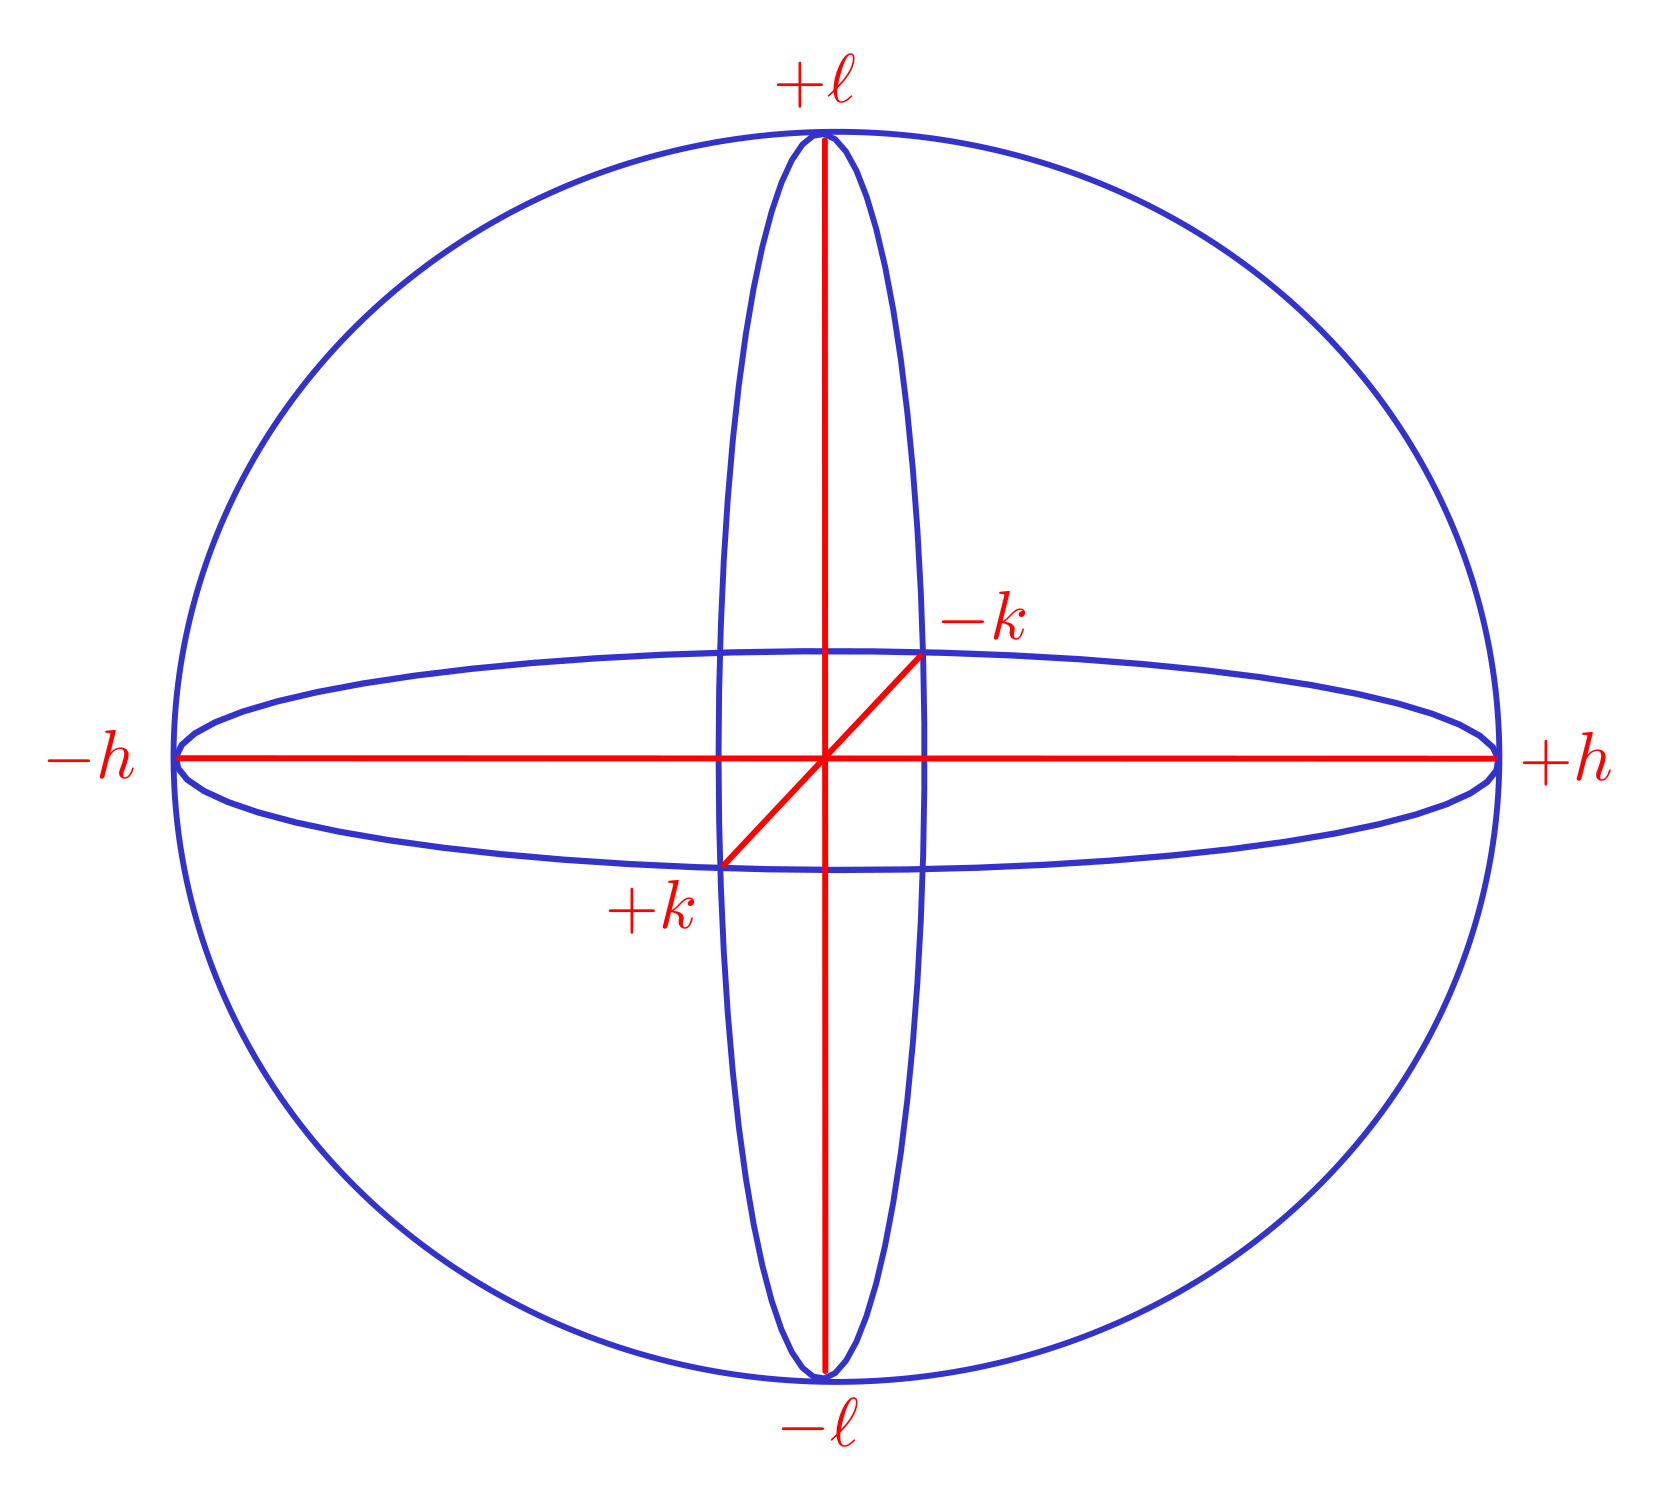
\includegraphics[scale=0.15]{full_sphere.png}
	\caption{\label{fig:full_sphere}Full sphere of data. All of $x$, $y$ and $z$ range from $-\infty$ through $0$ to $+\infty.$}
\end{figure}

A \textbf{full sphere of data} (figure~\ref{fig:full_sphere}) corresponds to%
%	
	\begin{itemize}%
%	
	    \item $h$ from $-\infty$ through $0$ to $+\infty,$
	    
	    \item $k$ from $-\infty$ through $0$ to $+\infty,$ and
	    
	    \item $\ell$ from $-\infty$ through $0$ to $+\infty.$
	    
	\end{itemize}
	
\begin{figure}
	\centering
	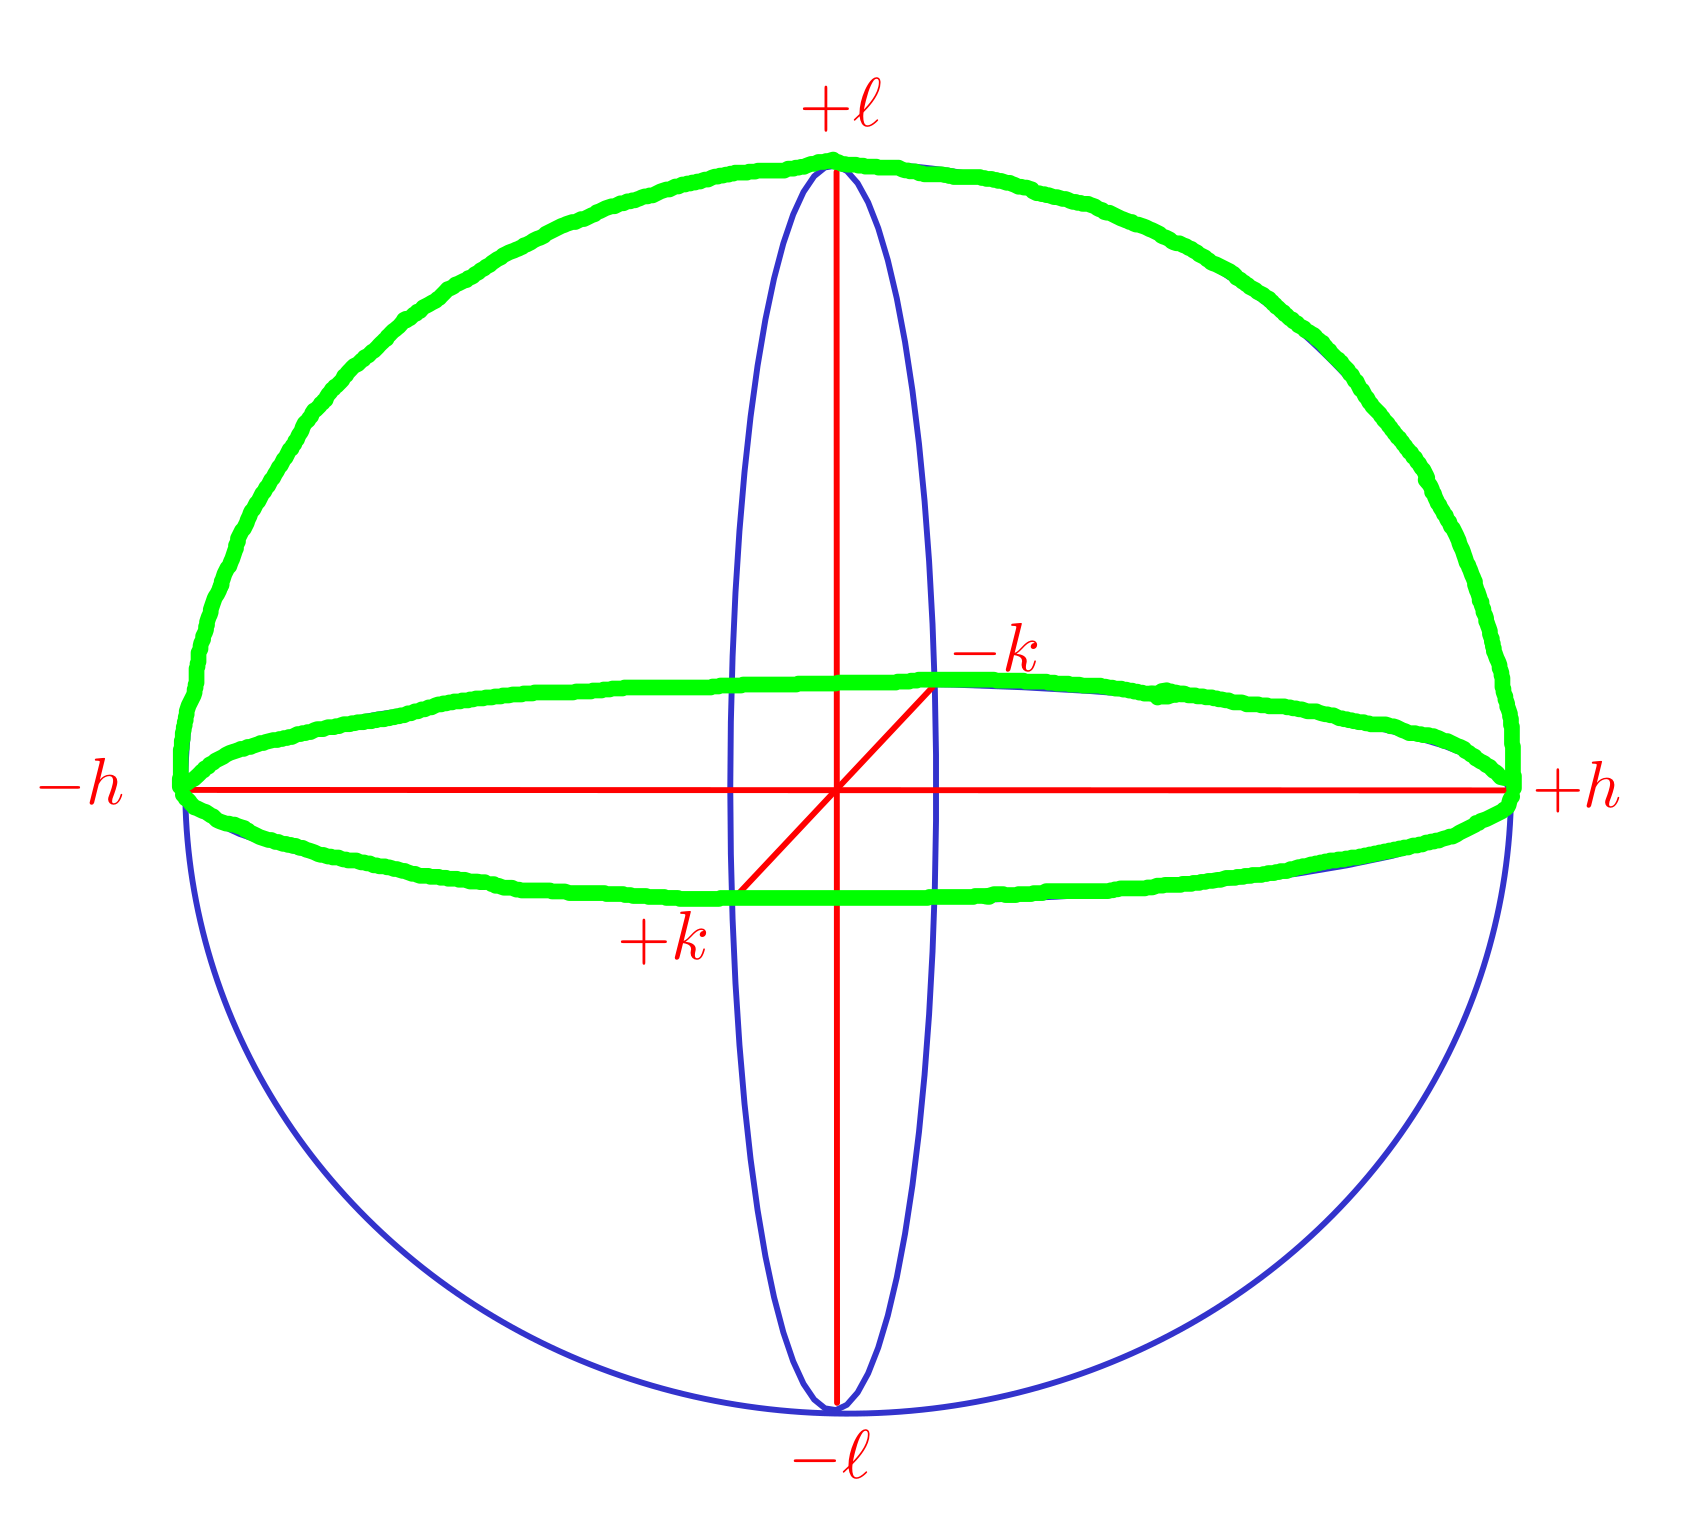
\includegraphics[scale=0.15]{hemisphere_data.png}
	\caption{\label{fig:hemisphere}A hemisphere of data corresponds to the closed region demarcated in green. The lower hemisphere is also equally valid due to Friedel's Law.}
\end{figure}
	
A \textbf{hemisphere of data} (figure~\ref{fig:hemisphere}) implies that one index among $h$, $k$ and $\ell$ will run from $0$ to $+\infty,$ and the other two indices will range from $-\infty$ through $0$ to $+\infty.$
	
The maximum \textbf{Laue symmetry} of a particular crystal system, combined with Friedel's law, tells us how much data is sufficient for a particular crystal system.

A \ul{triclinic system}, for instance, has only two possible crystallographic symmetries: $1$ and $\bar{1},$ and hence, the maximum Laue symmetry is $\bar{1}.$  This is basically a centre of inversion symmetry. Therefore, only Friedel's Law applies here, and we have to record only a hemisphere of data.

\begin{figure}
	\centering
	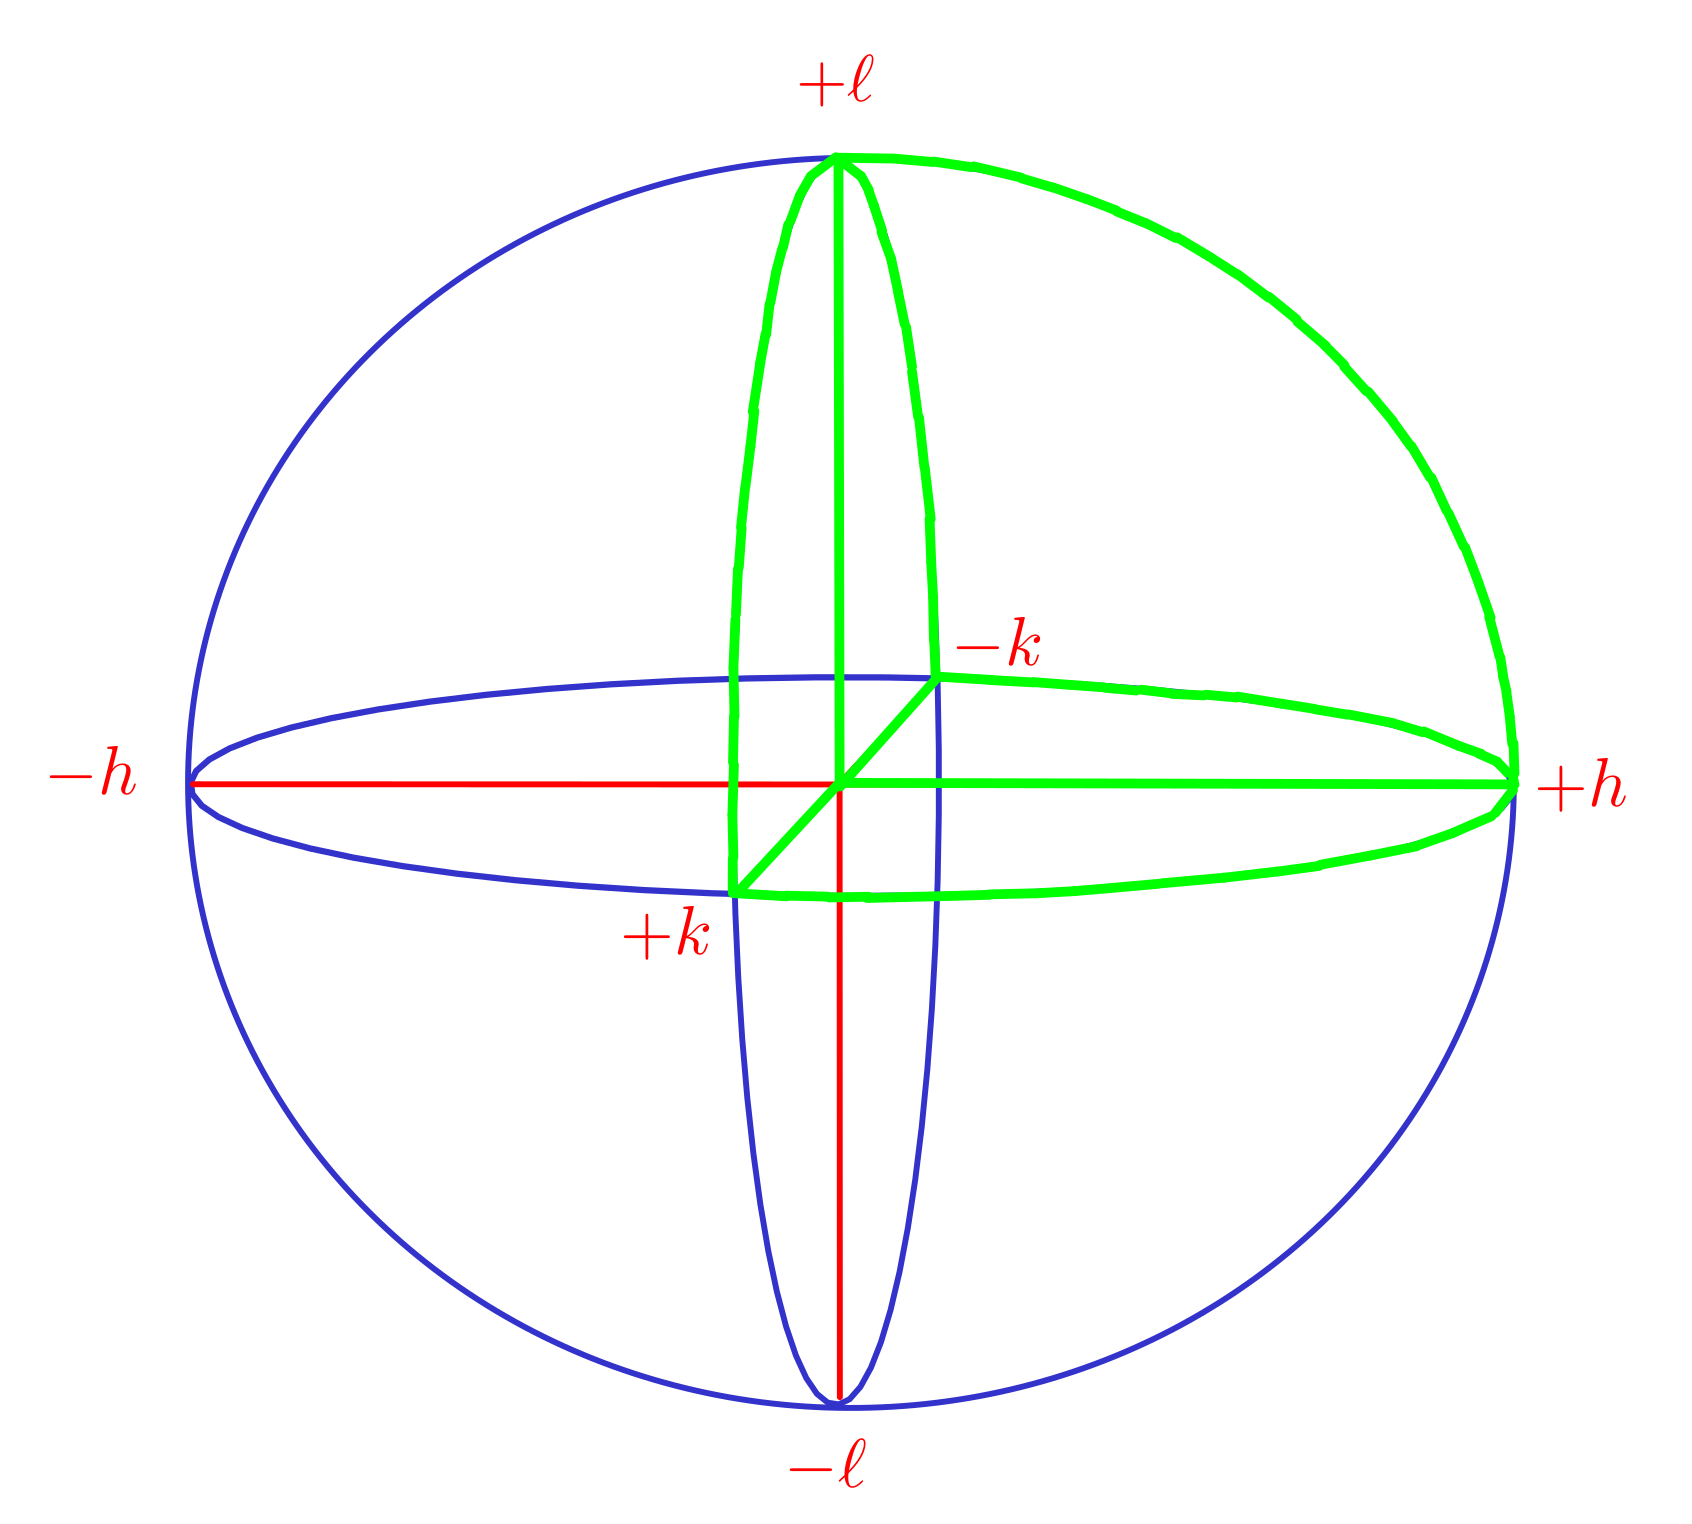
\includegraphics[scale=0.15]{one_fourth_sphere1.png}
	\caption{\label{fig:one_fourth_sphere}For a monoclinic system, only one-fourth data (the demarcated region) is sufficient.}
\end{figure}

For a \ul{monoclinic system}, the maximum Laue symmetry is $2/m,$ which is a 2-fold rotation axis, and a mirror plane $m \perp$ the rotation axis. If we consider $y$ to be the unique axis, such that $2 \parallel y$, then we have two sets of reflections:%
%	
\begin{equation}
\tikzmarknode[is]{a}{I}_{\tikzmarknode[is]{b}{h}kl}
    \equiv I_{\tikzmarknode[is]{c}{\bar{h}} \bar{k} \bar{\ell}}
    \equiv I_{\tikzmarknode[is]{d}{\bar{h}} \tikzmarknode[is]{e}{k} \bar{\ell}}
    \equiv I_{\tikzmarknode[is]{f1}{h} \tikzmarknode[is]{f}{\bar{k}} \ell}
\end{equation}
%
\begin{center}  % <--- for space of image
%
\begin{tikzpicture}[remember picture, overlay]
\draw[ ->, blue]          ([xshift=+1pt] b) |-|[distance=5mm]  (c.south) node[lbl, pos=0.5] {FL};
\draw[ ->, teal]    ([xshift=-1pt] b) |-|[distance=9mm]  (d.south) node[lbl, pos=0.6] {$2 \parallel y$};
\draw[ ->, purple]  ([xshift=+1pt] a) |-|[distance=15mm] (f.south) node[lbl, pos=0.65] {$m \perp y$};
%
\draw[ <->, blue]    (e.south) to[bend right=45, "FL" lbl=north] (f1.south);
\end{tikzpicture}
%
\vspace{10ex}        % <--- additional space for image
%
\end{center}
%	
and%
%
\begin{equation}
\tikzmarknode[is]{a}{I}_{\tikzmarknode[is]{b}{\bar{h}} k \ell}
    \equiv I_{\tikzmarknode[is]{c}{h} \bar{k} \bar{\ell}}
    \equiv I_{\tikzmarknode[is]{d}{h} \tikzmarknode[is]{e}{k} \bar{\ell}}
    \equiv I_{\tikzmarknode[is]{f1}{\bar{h}} \tikzmarknode[is]{f}{\bar{k}} \ell}
\end{equation}
%
\begin{center}  % <--- for space of image
%
\begin{tikzpicture}[remember picture, overlay]
\draw[ ->, blue]          ([xshift=+1pt] b) |-|[distance=5mm]  (c.south) node[lbl, pos=0.5] {FL};
\draw[ ->, teal]    ([xshift=-1pt] b) |-|[distance=9mm]  (d.south) node[lbl, pos=0.6] {$2 \parallel y$};
\draw[ ->, purple]  ([xshift=+1pt] a) |-|[distance=15mm] (f.south) node[lbl, pos=0.65] {$m \perp y$};
%
\draw[ <->, blue]    (e.south) to[bend right=45, "FL" lbl=north] (f1.south);
\end{tikzpicture}
%
\vspace{10ex}        % <--- additional space for image
%
\end{center}
%
where ``FL`` stands for Friedel's Law.

We only need to record one each from these two sets, and the minimum number of reflections required to be recorded is reduced to one-fourth, shown in figure~\ref{fig:one_fourth_sphere}. Thus, the range of $h,$ $k$ and $\ell$ is as follows:%
%	
	\begin{itemize}%
%	
	    \item $k \tendsto 0$ to $+\infty$ (as $y$ is the unique axis), \textit{and}
	    
	    \item $h \tendsto 0$ to $+\infty$ and $\ell \tendsto -\infty$ to $+\infty$, \textit{or}
	    
	    \item $h \tendsto -\infty$ to $+\infty$ and $\ell \tendsto 0$ to $+\infty.$
	    
	\end{itemize}

For an \ul{orthorhombic system}, the maximum Laue symmetry is $mmm \implies m \perp x,\ m \perp y,\ m \perp z.$ Thus, the following reflections are all equivalent:%
%
\begin{equation}
\tikzmarknode[is]{a}{I}_{\tikzmarknode[is]{b}{h}kl}
    \equiv I_{\tikzmarknode[is]{c}{\bar{h}} \bar{k} \bar{\ell}}
    \equiv I_{\tikzmarknode[is]{d}{\bar{h}} \tikzmarknode[is]{e}{k} \ell}
    \equiv I_{h \tikzmarknode[is]{f}{\bar{k}} \bar{\ell}}
    \equiv \tikzmarknode[is]{g}{I}_{h \bar{k} \tikzmarknode[is]{h}{\ell}}
    \equiv I_{\bar{h} k \tikzmarknode[is]{i}{\bar{\ell}}}
    \equiv \tikzmarknode[is]{j}{I}_{h k \tikzmarknode[is]{k}{\bar{\ell}}}
    \equiv I_{\bar{h} \tikzmarknode[is]{l}{\bar{k}} \ell}
\end{equation}
\begin{center}  % <--- for space of image
\begin{tikzpicture}[remember picture, overlay]
\draw[ ->, blue]          ([xshift=+1pt] b) |-|[distance=5mm]  (c.south) node[lbl, pos=0.5] {FL};
\draw[ ->, teal]    ([xshift=-1pt] b) |-|[distance=9mm]  (d.south) node[lbl, pos=0.6] {$m \perp x$};
\draw[ ->, purple]  ([xshift=+1pt] a) |-|[distance=13mm] (g.south) node[lbl, pos=0.65] {$m \perp y$};
\draw[ ->, orange]  ([xshift=-1pt] a) |-|[distance=18mm] (j.south) node[lbl, pos=0.7] {$m \perp z$};
%
\draw[ <->, blue]    (e.south) to[bend right=45, "FL" lbl=north] (f.south);
\draw[ <->, blue]    (h.south) to[bend right=45, "FL" lbl=north] (i.south);
\draw[ <->, blue]    (k.south) to[bend right=45, "FL" lbl=north] (l.south);
\end{tikzpicture}
\vspace{10ex}        % <--- additional space for image
\end{center}
%
and we need to record only one from this set. Thus, the data to be recorded decreases to one-eighth for an orthorhombic system, and we need to only record the region highlighted in figure~\ref{fig:one_eighth_sphere}.

\begin{figure}
	\centering
	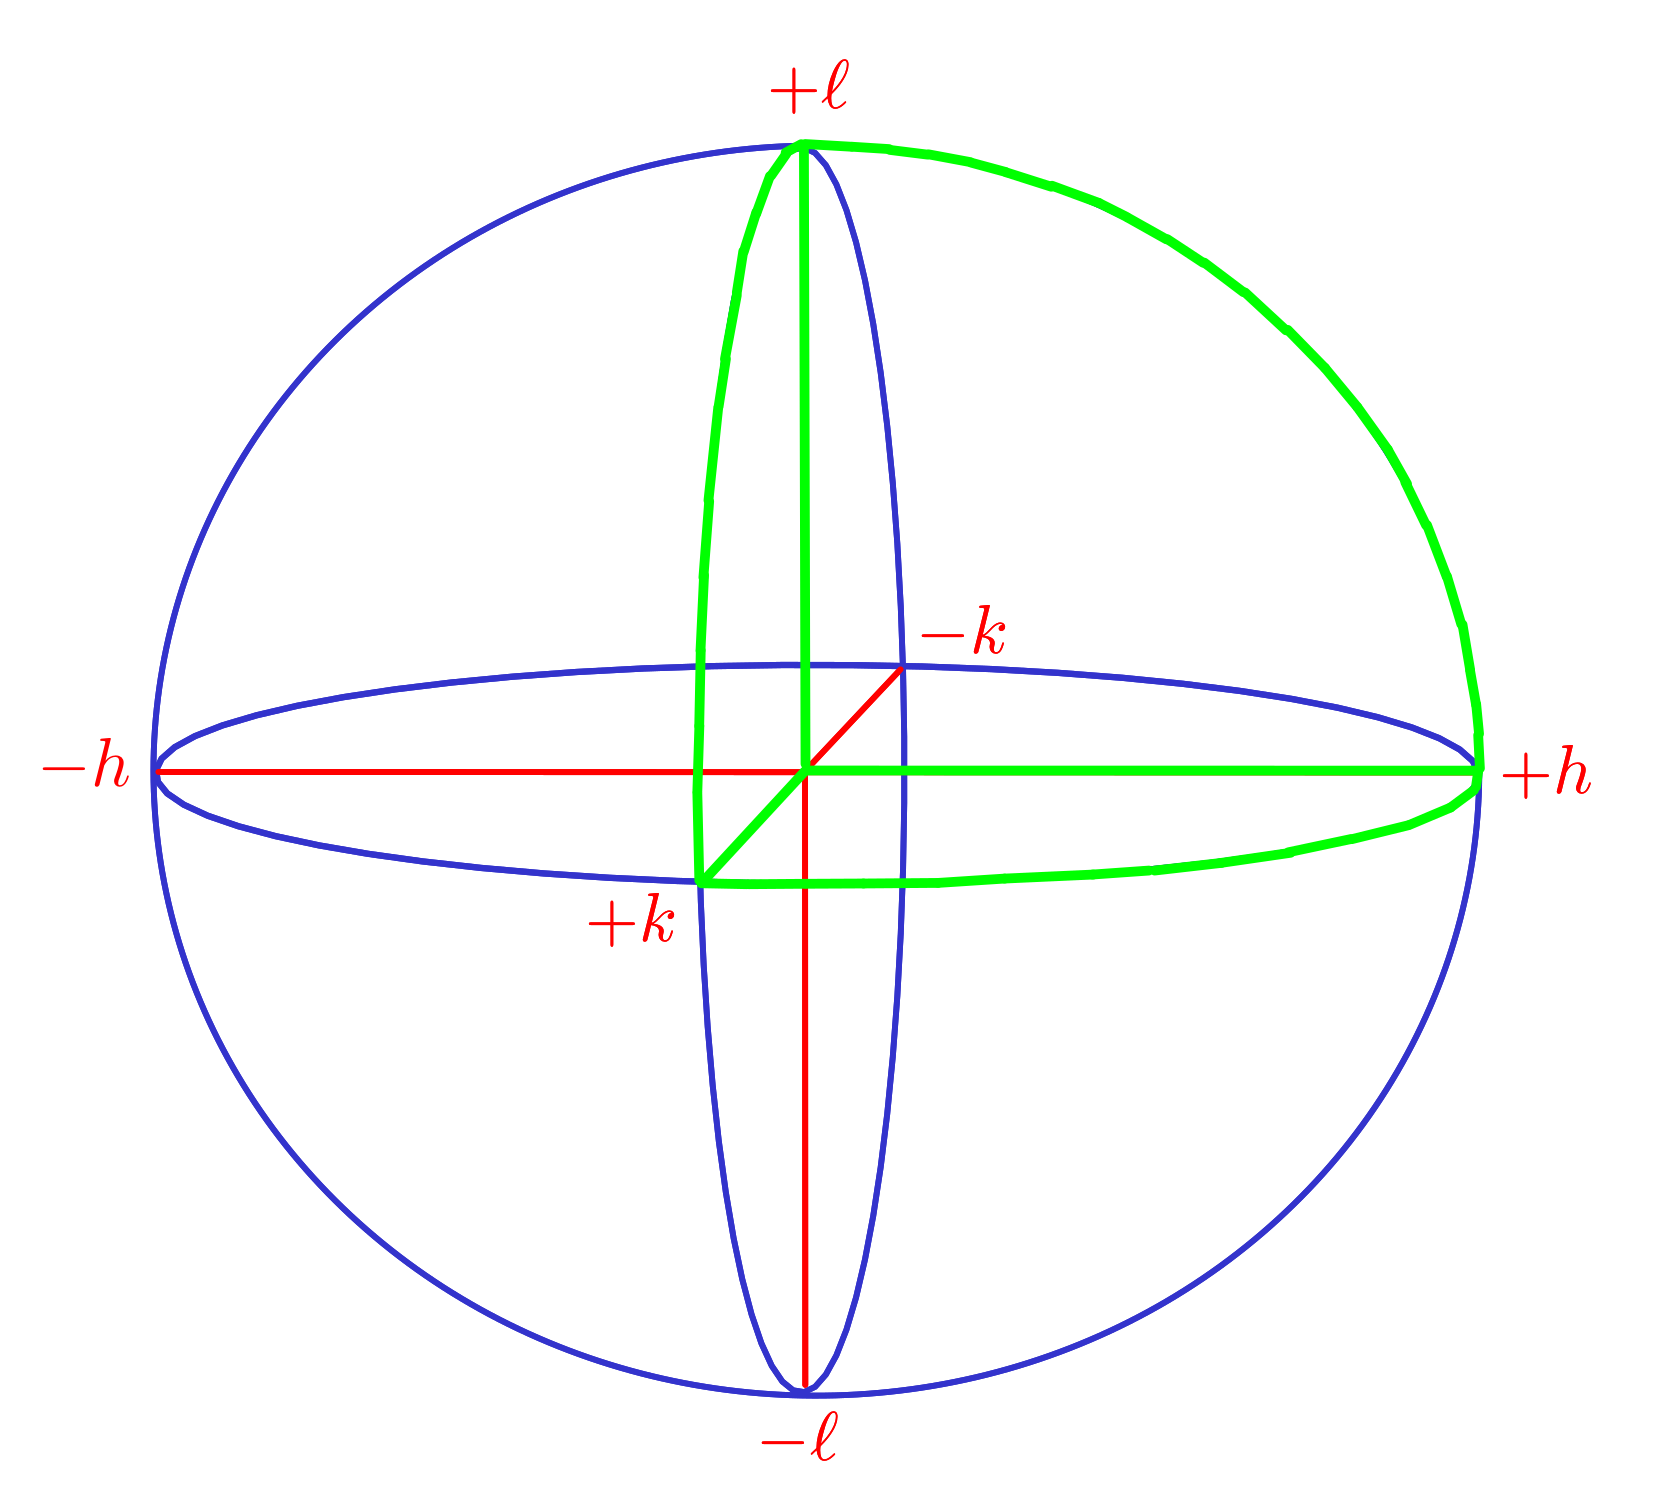
\includegraphics[scale=0.15]{one_eighth_sphere.png}
	\caption{\label{fig:one_eighth_sphere}For an orthorhombic system, only one-eighth sphere data (the region demarcated in green) is sufficient.}
\end{figure}

Understanding how much data we have to collect for different crystal systems was extremely essential even, say, 20 years back. In those days, the detector in the diffractometer used to be a point detector. Such a detector can record only one reflection at a time, and it would take quite a long time to center a reflection at the maxima and then record the intensity. 

When we mount a crystal on the diffractometer and rotate it about the $\phi$ axis, diffraction would be visible from all directions. The detector, however, being a point detector, could only measure in a particular plane. The procedure used was as follows: First, the detector would be moved to the location of a particular reflection. Next, the detector would be moved in very small steps to locate the maxima of the diffracted light. Thereafter, the crystal would be very slowly rotated about the different axes of the diffractometer to maximize the intensity once again. Thus, for recording a particular reflection, it would take 5-7 minutes. If the intensity is weak at that point, it would take at least 15 minutes to get sufficient data. So, without Friedel's Law, one would have to spend more than a week to record all reflections.

Suppose, for a tricilinic system, 10,000 reflections are possible considering all $(hk\ell)$ and $(\bar{h} \bar{k} \bar{\ell}).$ It would take around 6-8 days for this data to be collected. Thanks to Friedel's Law, we know that we have to collect only half of the data rather than the full sphere. If we know whether the crystal is monoclinic, triclinic or orthorhombic, data collection time reduces further.

Even with the advent of modern area detectors, Friedel's Law is still equally useful.